%%%%%%%%%%%%%%%%%%%%%%%%%%%%%%%%%%%%%%%%%%%%%%%%%%%%%%%%%%%%%%%%%%%%%%%%%%%%
% Capa
% Este arquivo gera a primeira página do BoletIME.
% No geral, não é necessário editá-lo. Para configurar os textos da primeira
% página, vá ao arquivo "/sumario.tex".
%%%%%%%%%%%%%%%%%%%%%%%%%%%%%%%%%%%%%%%%%%%%%%%%%%%%%%%%%%%%%%%%%%%%%%%%%%%%

%%%%%%%%%%%%%%%%%%%%%%%%%%%%%%%%%%%%%%
% Fundo com a imagem (cabeçalho
%%%%%%%%%%%%%%%%%%%%%%%%%%%%%%%%%%%%%%
\begin{textblock*}{\paperwidth}(0cm,0.4cm)
    \centering
    
\includegraphics[width=0.95\paperwidth]{img/boletime_cabecalho.png}\\
\end{textblock*}

%%%%%%%%%%%%%%%%%%%%%%%%%%%%%%%%%%%%%%
% Texto e linha vermelha
%%%%%%%%%%%%%%%%%%%%%%%%%%%%%%%%%%%%%%
\begin{textblock*}{\paperwidth}(0.5cm,0.275\paperheight)
    \textls[85]{
    \sffamily\bfseries
        produção do centro acadêmico da matemática, estatística e computação 
    \hspace{0.3cm} \textbar{} \hspace{1.1cm}
    \MakeLowercase{\mes}.\ano}\\    
    \textcolor{vermelho_camat}{\rule{0.95\paperwidth}{0.25cm}} % Largura e espessura do risco
\end{textblock*}

%%%%%%%%%%%%%%%%%%%%%%%%%%%%%%%%%%%%%%
% Texto no canto superior direito (nº edicao)
%%%%%%%%%%%%%%%%%%%%%%%%%%%%%%%%%%%%%%
\begin{textblock*}{5cm}(15cm, 1cm)
    \raggedleft 
    {\huge \archivoblack {nº \edicao}}
\end{textblock*}

% Espaçamento
\vspace*{0.2\paperheight}

%%%%%%%%%%%%%%%%%%%%%%%%%%%%%%%%%%%%%%
% Sumário
%%%%%%%%%%%%%%%%%%%%%%%%%%%%%%%%%%%%%%
\begin{multicols}{2}
    %%%%%%%%%%%%%%%%%%%%%%%%%%%%%%%%%%%%%%%%%%%%%%%%%%%%%%%%%%%%%%%%%%%%%%%%%%%%
% Sumário (1ª página)
% Este arquivo contém os textos exibidos na primeira página. Edite-o conforme
% for necessário. Por padrão, a seção é dividida em duas colunas, e estas não
% dividem o texto automaticamente entre si, então é necessário definir
% explicitamente o que está em cada coluna.
%%%%%%%%%%%%%%%%%%%%%%%%%%%%%%%%%%%%%%%%%%%%%%%%%%%%%%%%%%%%%%%%%%%%%%%%%%%%

% Tamanho da fonte. Pitititica
\footnotesize

\noindent\begin{minipage}[t][0.20\paperheight][t]{\columnwidth}
%%%%%%%%%%%%%%%%%%%%%%%%%%%%%%%%%%%%%%%%%%%%%%%%%%%%%%%%%%%%%%%%%%%%%%%%%%%%
%%% > O TEXTO DA PRIMEIRA COLUNA VAI AQUI
%%%%%%%%%%%%%%%%%%%%%%%%%%%%%%%%%%%%%%%%%%%%%%%%%%%%%%%%%%%%%%%%%%%%%%%%%%%%

\itemSumario{Falta de água no IME}{
Envio de um convite para refletir sobre as diferentes realidades presentes
no IME na forma de um relato sobre como é estudar de dia e de noite.
}{2}

\itemSumario{Duchamp e Tarsila}{
Uma respota ao “Mas isto até eu faço!” da edição 10 do BoletIME.
}{3}


\itemSumario{Sessão Poesias}{
Poesia encontrada na parede do banheiro da sede do DCE Livre da USP.
}{4}


\itemSumario{Sobre carta da Comissão de Recepção}{
Crítica enviada sobre a maneira como o tema da Comissão de Recepção 2024 foi conduzida.
}{5}


\itemSumario{Novo projeto acadêmico para o próximo ciclo}{
Um convite para entender o que é um projeto acadêmico, onde o IME se encontra nisso, e como a comunidade como um todo pode e deve participar da sua construção. Foi marcada a 1ª reunião aberta do projeto acadêmico para 06 de junho, às 17h no saguão do Bloco B.
}{7}

%%%%%%%%%%%%%%%%%%%%%%%%%%%%%%%%%%%%%%%%%%%%%%%%%%%%%%%%%%%%%%%%%%%%%%%%%%%%
%%% > O TEXTO DA PRIMEIRA COLUNA TERMINA AQUI
%%%%%%%%%%%%%%%%%%%%%%%%%%%%%%%%%%%%%%%%%%%%%%%%%%%%%%%%%%%%%%%%%%%%%%%%%%%%
\end{minipage}

\columnbreak

\noindent\begin{minipage}[t][0.20\paperheight][t]{\columnwidth}
%%%%%%%%%%%%%%%%%%%%%%%%%%%%%%%%%%%%%%%%%%%%%%%%%%%%%%%%%%%%%%%%%%%%%%%%%%%%
%%% > O TEXTO DA SEGUNDA COLUNA VAI AQUI
%%%%%%%%%%%%%%%%%%%%%%%%%%%%%%%%%%%%%%%%%%%%%%%%%%%%%%%%%%%%%%%%%%%%%%%%%%%%

\itemSumario{DCE Livre da USP: chapa Fazer Valer a Luta eleita para o mandato 2024/2025}{
Confira os resultados e estatísticas das eleições do DCE Livre da USP 2024.
}{8}

\itemSumario{Efeito da redução da jornada sobre os salários}{
Trecho do segundo capítulo do livro Salário, preço e lucro, de Karl Marx.
}{9}

\vspace{1cm}

\quadradao{\LARGE}
{1.4}
{50}
{.9\textwidth}
{vermelho_camat}
{0.2cm}{
- É pavê ou pacumê?\\
- Sim.}

% gorrinho natalinho no bloco
\begin{textblock*}{5cm}(18cm, 15.3cm)
    
\includegraphics[width=0.5\linewidth]{textos//img/gorro.png}
\end{textblock*}

%%%%%%%%%%%%%%%%%%%%%%%%%%%%%%%%%%%%%%%%%%%%%%%%%%%%%%%%%%%%%%%%%%%%%%%%%%%%
%%% > O TEXTO DA SEGUNDA COLUNA TERMINA AQUI
%%%%%%%%%%%%%%%%%%%%%%%%%%%%%%%%%%%%%%%%%%%%%%%%%%%%%%%%%%%%%%%%%%%%%%%%%%%%
\end{minipage}
\end{multicols}

%%%%%%%%%%%%%%%%%%%%%%%%%%%%%%%%%%%%%%
% Imagem de divulgação do BoletIME
%%%%%%%%%%%%%%%%%%%%%%%%%%%%%%%%%%%%%%
\begin{textblock*}{\paperwidth}(0cm, 0.82\paperheight)
    \centering
    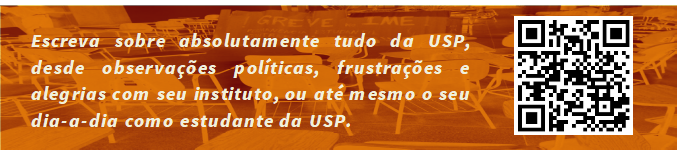
\includegraphics[width=0.95\paperwidth]{img/qr_code.png}
\end{textblock*}